% -*- coding: utf-8 -*-

\chapter{Estado del Arte}\label{ch:estado}

\section{Navegación, planificación de trayectorias y control reactivo}
Un aspecto esencial de un robot móvil es su capacidad de navegación. Sin entrar en profundidad en la cinemática implicada en el movimiento de diferentes tipos de robots móviles, ha de tenerse en cuenta que ésta limita significativamente las posibles configuraciones que puede adoptar un robot para moverse entre dos determinados puntos. El término \emph{trayectoria} se diferencia del de \emph{camino} en que incorpora la dimensión tiempo. Así, mientras que en un camino se tiene una serie discreta de puntos o configuraciones, en una trayectoria se asocia a cada uno de ellos una velocidad. No obstante, cuando se hace referencia a la planificación, es corriente el empleo de ambos conceptos indistintamente.

\subsection{Control de movimiento}
El desplazamiento del robot entre dos puntos se realiza mediante lo que se conoce como \emph{motion control}. Existen diferentes técnicas para afrontar esta tarea, distinguiéndose entre control en bucle abierto o control con realimentación\cite{Siegwart04}.
\subsubsection{Control en bucle abierto}
Consiste en el seguimiento de una trayectoria definida por un perfil de puntos o velocidades en función del tiempo. El mayor inconveniente que presenta es la alta probabilidad de que el robot no llegue a su destino si por algún motivo se encuentra en un lugar distinto al previamente esperado para un cierto momento. Además, precalcular una trayectoria posible no resulta sencillo en muchos casos. Otra de sus desventajas es que suele basarse en movimientos de giro o avance puros, y con frecuencia da lugar a movimientos algo bruscos.
\subsubsection{Control con realimentación}
Una manera más apropiada de tratar el control de movimiento de un robot móvil es el control mediante \emph{feedback} de su posición. Con un controlador de este tipo, la planificación de trayectorias se reduce a la obtención de una serie de puntos intermedios que determinen el camino a seguir entre los puntos origen y destino.

\subsection{Aptitudes para la navegación: planificación y\\ reacción}
En navegación de alto nivel juegan un papel fundamental las habilidades de planificación y reacción del robot. Ambos sistemas son igualmente importantes y han de integrarse adecuadamente. De nada sirve que el robot disponga de un conjunto de acciones a realizar para alcanzar un objetivo dado (plan), si durante la ejecución del mismo se encuentra con condiciones no previstas a las que no sabe cómo hacer frente. Tampoco tiene sentido que el robot sea capaz de reaccionar ante diferentes circunstancias si no puede guiarse para llegar al destino deseado. La solución teórica ideal lleva a la fusión de ambos conceptos, de modo que constantemente se elabora o actualiza un plan que reaccione en tiempo real a la información más inmediata que se tenga para describir el entorno.

Se dice que el sistema de un robot es completo si y sólo si para todos los posibles problemas que puedan encontrarse (diferentes estados de partida, mapas o destinos\ldots), cuando exista alguna trayectoria entre el estado inicial y el final, el sistema llegará al estado final. Por lo tanto, si un sistema es incompleto significa que existe al menos un problema que tiene solución para el cual el sistema no encuentra solución. Siendo una propiedad enormemente difícil de conseguir, a menudo se renuncia a la completitud por razones de coste computacional.

\subsubsection{Planificación de trayectorias}
La planificación de trayectorias se lleva a cabo en la mayoría de los casos en una representación formal denominada \emph{espacio de configuración}. Para un robot con $k$ grados de libertad, cada uno de sus posibles estados o configuraciones se describirá con $k$ valores reales: $q_{1},q_{2}...,q_{k}$. El vector que contenga esas $k$ coordenadas podrá considerarse como un punto en un espacio de dimensión $k$ que recibe el nombre de espacio de configuración $C$ del robot. En el caso de que el robot se mueva en las cercanías de algún obstáculo, han de evitarse las colisiones con él, lo cual puede complicarse mucho en el espacio físico. Sin embargo, en el espacio de configuración la resolución del problema es directa si se define el \emph{espacio de configuración de obstáculos} $O$ como el subespacio de $C$ en el que el robot choca contra algún objeto. El subespacio libre en el que el robot puede moverse con seguridad será la diferencia $F = C-O$.

Generalmente, se considera al robot móvil como un simple punto. En consecuencia, el espacio de configuración es fácilmente manejable por ser plano con ejes $x$ e $y$. Una importante consideración a realizar es el hecho de que al reducirse el robot a un punto, habrá que aumentar el tamaño de los obstáculos en la medida del radio del robot.

Una vez introducido este concepto, se distinguen tres estrategias principales para efectuar la planificación de trayectorias básica:
\begin{itemize}
  \item \emph{Mapa de líneas}: basado en identificar rutas en el espacio libre. Destacan los métodos del \emph{Gráfico de visibilidad } y del \emph{Diagrama de Voronoi}.
  \item \emph{Descomposición en celdillas}: a partir de una mapa de celdillas se clasifican éstas en libres y ocupadas y se crea un grafo de conectividad entre celdas libres adyacentes (ver \ref{mapas}).
  \item \emph{Campo de potencial}: consiste en imponer una adecuada función matemática sobre el espacio. Permite obtener la \emph{fuerza} sobre el robot (que se traducirá en una velocidad) como resultado de potenciales de atracción y repulsión.
\end{itemize}

Las trayectorias generadas por estos algoritmos pueden ser mejoradas en relación a distintos criterios. Por ejemplo, puede resultar interesante suavizar los ángulos en las trayectorias previas mediante arcos de circunferencia (como se implementa en el presente proyecto) o interpolación cuadrática. Estas técnicas de perfeccionamiento son también un componente relevante del término planificación de trayectorias.

\subsubsection{Control reactivo}
El control reactivo tiene como principal propósito evitar que el robot pueda chocar con algún obstáculo en el seguimiento de la trayectoria previamente hallada. Para ello existen diversos algoritmos que modifican estas trayectorias en función de los objetos detectados por las medidas que le llegan al robot procedentes de los sensores estereoceptivos. La presencia de obstáculos en una trayectoria obtenida mediante planificación sobre un mapa del entorno puede deberse a errores en la localización, a imprecisiones en el mapa utilizado o a obstáculos dinámicos no contemplados en dicho mapa.

Algunas soluciones (por ejemplo la mostrada en \cite{Feiten94}) consisten en calcular un conjunto de comandos de giro o de variación de la velocidad a aplicar al robot en función de lo que éste percibe a través de sus sensores. También se ha afrontado la tarea de esquivar obstáculos mediante controladores basados en lógica borrosa.

Un nuevo enfoque, efectivo y genérico, es el que se presenta en \cite{Lamiraux04}. A partir de un camino inicial libre de obstáculos, se trata de ir deformándolo iterativamente cuando se encuentran obstáculos próximos, siguiendo para ello un criterio de optimización. El camino deformado debe apartarse de los obstáculos, cumplir las restricciones cinemáticas de movimiento (lo que complica significativamente el problema en el caso de robots no holónomos) y mantener las mismas configuraciones inicial y final que el camino original. En el artículo se establece un marco teórico en el que la deformación del camino inicial se modela como un sistema dinámico dentro del algoritmo que controla el proceso.

También cabe mencionar que existen otros algoritmos de control reactivo que podrían considerarse más avanzados por tener en cuenta la velocidad de los obstáculos detectados. No obstante, emplean modelos excesivamente sencillos del robot y los obstáculos que no suelen conducir a un buen comportamiento práctico.

Por último, hay trabajos recientes que se centran en resolver el problema en escenarios complejos, con un alto grado de ocupación o dinámicos. Para ello, se basan en estrategias de “divide y vencerás” y posteriormente aplican diferentes técnicas de control reactivo. En \cite{Minguez04} se explica una metodología que, a nivel simbólico, consiste en identificar situaciones para posteriormente aplicar una determinada acción en cada caso. Una vez definidas las posibles situaciones (a partir de las posiciones relativas de robot, obstáculos y destino) así como las acciones asociadas a las mismas, se realiza una implementación geométrica particular.

\section{Localización y construcción de mapas con un robot móvil}
Uno de los mayores problemas que conciernen a la navegación de robots móviles consiste en la determinación de su localización con un elevado grado de precisión. Para cumplir con el objetivo de autonomía no basta con situar el robot en un sistema de referencia global sino que es imprescindible conocer su posición relativa tanto respecto a posibles obstáculos móviles como respecto al modelo estático de su entorno. Para ello, existen diferentes alternativas utilizando mapas que, o bien se introducen previamente al robot, o bien se elaboran a medida que el mismo se mueve por un determinado lugar. Esta segunda opción empieza a desarrollarse a finales de los años 80. En un principio se desacoplaron los problemas de construcción del mapa y de la localización del robot en el mismo; pronto se descubriría que la solución rigurosa requiere tratar ambos aspectos al mismo tiempo en lo que se conoce como SLAM (Simultaneous Localization and Mapping). La solución al problema SLAM está considerada como pieza clave en la búsqueda de la completa autonomía de un robot móvil y concentra los principales esfuerzos de investigación de grupos de robótica móvil de todo el mundo que han conseguido importantes avances y continúan intentando resolver dicho problema.

El origen de las dificultades en la localización y la construcción de mapas se deriva de la existencia de ruido en las medidas de los sensores y en las limitaciones en el rango de las mismas. Un poco más en profundidad, los principales factores que impiden que el proceso sea más sencillo son los siguientes:
\begin{itemize}
  \item  Las observaciones se obtienen con respecto al sistema de referencia propio del robot, cuya posición viene afectada de un cierto grado de incertidumbre inherente a la odometría. Así, la imprecisión en las observaciones se añade a la ya existente en la posición del robot y se complica extremadamente la minimización de los errores.
  \item En multitud de casos es necesaria la representación de mapas de tamaño grande, lo cual supone un mayor coste computacional y una mayor imprecisión en la odometría según aumentan los desplazamientos del robot.
  \item Los entornos suelen ser dinámicos, sobre todo en el caso de robots guía o domésticos. Si se considera que las observaciones corresponden a puntos fijos representados con carácter permanente en el mapa se simplifica el problema, pero se tienen discrepancias con la realidad. Una aproximación parcialmente eficiente consiste en ir borrando objetos transitorios del mapa a lo largo del tiempo, tratándolos a modo de ruido. El rápido avance de la visión artificial y el desarrollo de dispositivos sensores que diferencien entre obstáculos móviles y estructuras estáticas dentro de un marco de referencia móvil permitirán notables mejoras en este aspecto.
  \item La asociación de las observaciones con los objetos del mapa puede resultar compleja si éstos son parecidos entre sí. En muchos casos no puede efectuarse la correspondencia de forma determinista y ha de emplearse una formulación probabilista. Algunas mejoras para abordar este problema y descartar las asociaciones erróneas se han presentado en \cite{Rodriguez-Losada07}.
  \item Los entornos son tridimensionales pero contemplar este aspecto introduce un mayor grado de complejidad y ha de tenerse en cuenta que generalmente los sensores están configurados para una percepción plana horizontal. Aunque existen algunos trabajos en la representación de mapas tridimensionales, la mayor parte de los algoritmos más empleados hasta el momento aceptan la hipótesis de bidimensionalidad del entorno. El paso a modelos en tres dimensiones es uno de los próximos objetivos a seguir (capítulo \ref{ch:conclusiones}).
\end{itemize}

\subsection{Tipos de mapas}\label{mapas}
Cuanto mayor sea la complejidad del mapa a emplear, mayor será la complejidad computacional de su construcción, de la localización y de la navegación. La precisión del mapa vendrá condicionada en cada caso por la precisión que se necesite en el movimiento del robot y por la precisión de los sensores de que se disponga.

Se establecen tres niveles posibles de representación en la definición de un mapa: geométrico, topológico y semántico. Una representación completa del entorno debería incorporarlos todos pero con frecuencia las soluciones halladas se centran en uno sólo de ellos y, a lo sumo, incluyen uno o los dos restantes como mera información extra que pueda mejorar la navegación.

El nivel métrico consiste en representar las coordenadas y propiedades de los objetos del mapa. Este modelo puede a su vez ser geométrico, en el que se representan elementos discretos del entorno de modo que almacenan su parametrización geométrica, o discretizado, en el que la ocupación del entorno se analiza mediante una división del mismo.
Así, los mapas métricos geométricos representan objetos con determinadas características geométricas y diferentes grados de complejidad dependiendo de las capacidades sensoriales y de extracción de información. En la figura \ref{fg:geometricos} se muestran dos mapas geométricos que reflejan propiedades características de los entornos de interiores. En el mapa de la izquierda se representan las paredes mediante segmentos y en el de la derecha puede apreciarse que las esquinas y objetos delgados, como patas de mobiliario, se representan como puntos.

\begin{figure}[hbt]
  \centering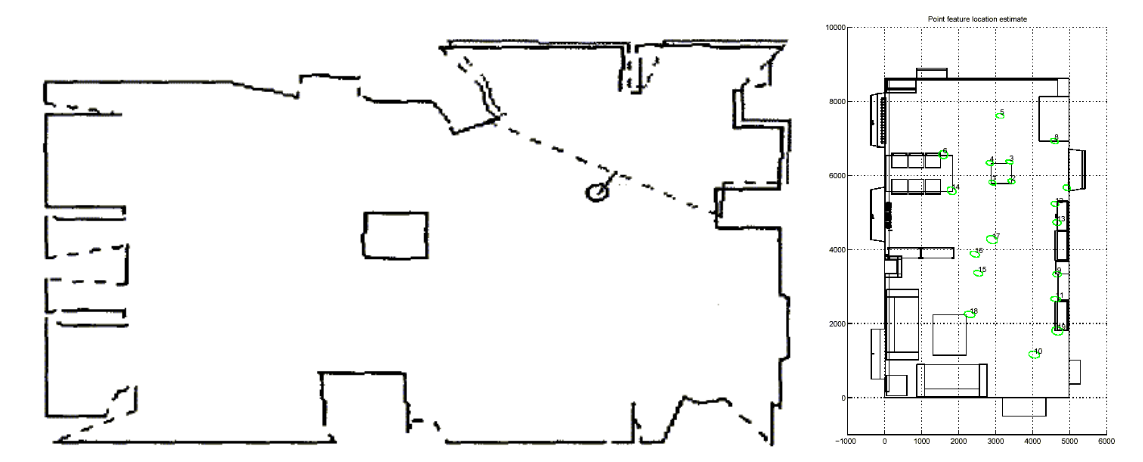
\includegraphics[width=0.5\textwidth]{mapas_geometricos}\\
  \caption{Mapas métricos geométricos}\label{fg:geometricos}
\end{figure}

Este tipo de mapas es ampliamente utilizado en entornos estructurados debido principalmente a la facilidad de visualización que ofrecen y la compacidad que presentan. Otra ventaja fundamental es la filtración de los objetos dinámicos al hacerse la extracción previa de características del entorno. Los sensores necesarios para construir estos mapas no pueden generar mucho ruido, puesto que han de permitir distinguir los diferentes elementos del entorno. Otro inconveniente a resaltar es su incapacidad para proporcionar un modelo completo del espacio que rodea al robot. Los puntos que no se identifican como características geométricas del mundo real son eliminados, con lo que para ganar en robustez y compacidad se pierde información de los sensores. Esta limitación afecta a tareas como la planificación de trayectorias y la exploración de entornos, reduciendo consiguientemente la utilidad de estos mapas en la navegación de robots móviles.

En los mapas métricos discretizados,se utiliza la información de los sensores sin segmentar y se construye una función de densidad de probabilidad de ocupación del espacio. Como ésta no puede cubrir todo el espacio de forma continua, se efectúa una descomposición en celdillas y se asigna una probabilidad a que cada una esté ocupada o libre. Esta división puede ser exacta, manteniendo las fronteras de los obstáculos como bordes de las celdillas, o mediante celdillas de dimensiones fijas que se reparten por todo el espacio \cite{Siegwart04}. En las figuras \ref{fg:exactas} y \ref{fg:fijas} pueden verse ejemplos de ambos tipos de descomposición. En la división en celdillas fijas se aprecia que un estrecho paso entre dos obstáculos puede perderse con esta representación.

 \begin{figure}[hbt]
  \centering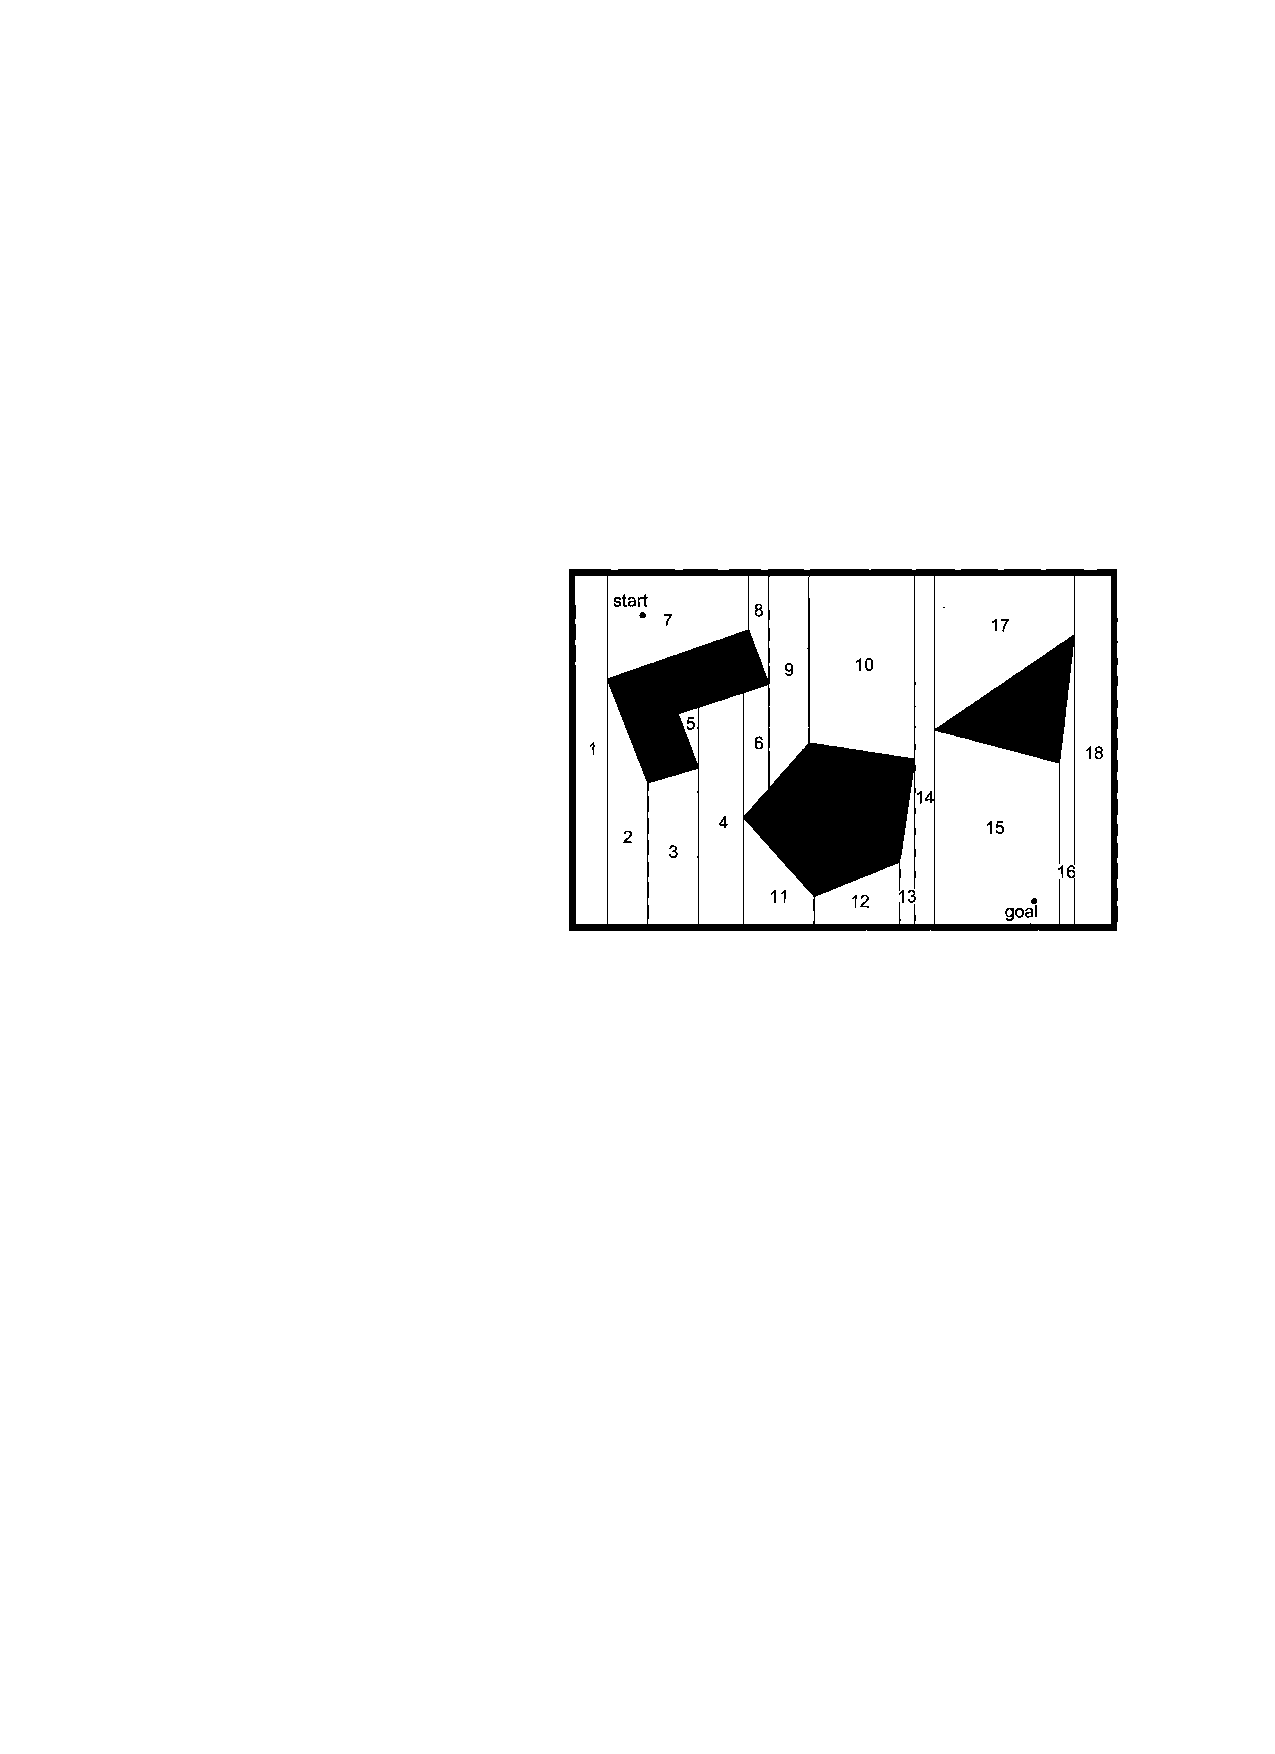
\includegraphics[width=0.5\textwidth]{celdas_exactas}\\
  \caption{Descomposición en celdillas exactas}\label{fg:exactas}
\end{figure}

\begin{figure}[hbt]
  \centering{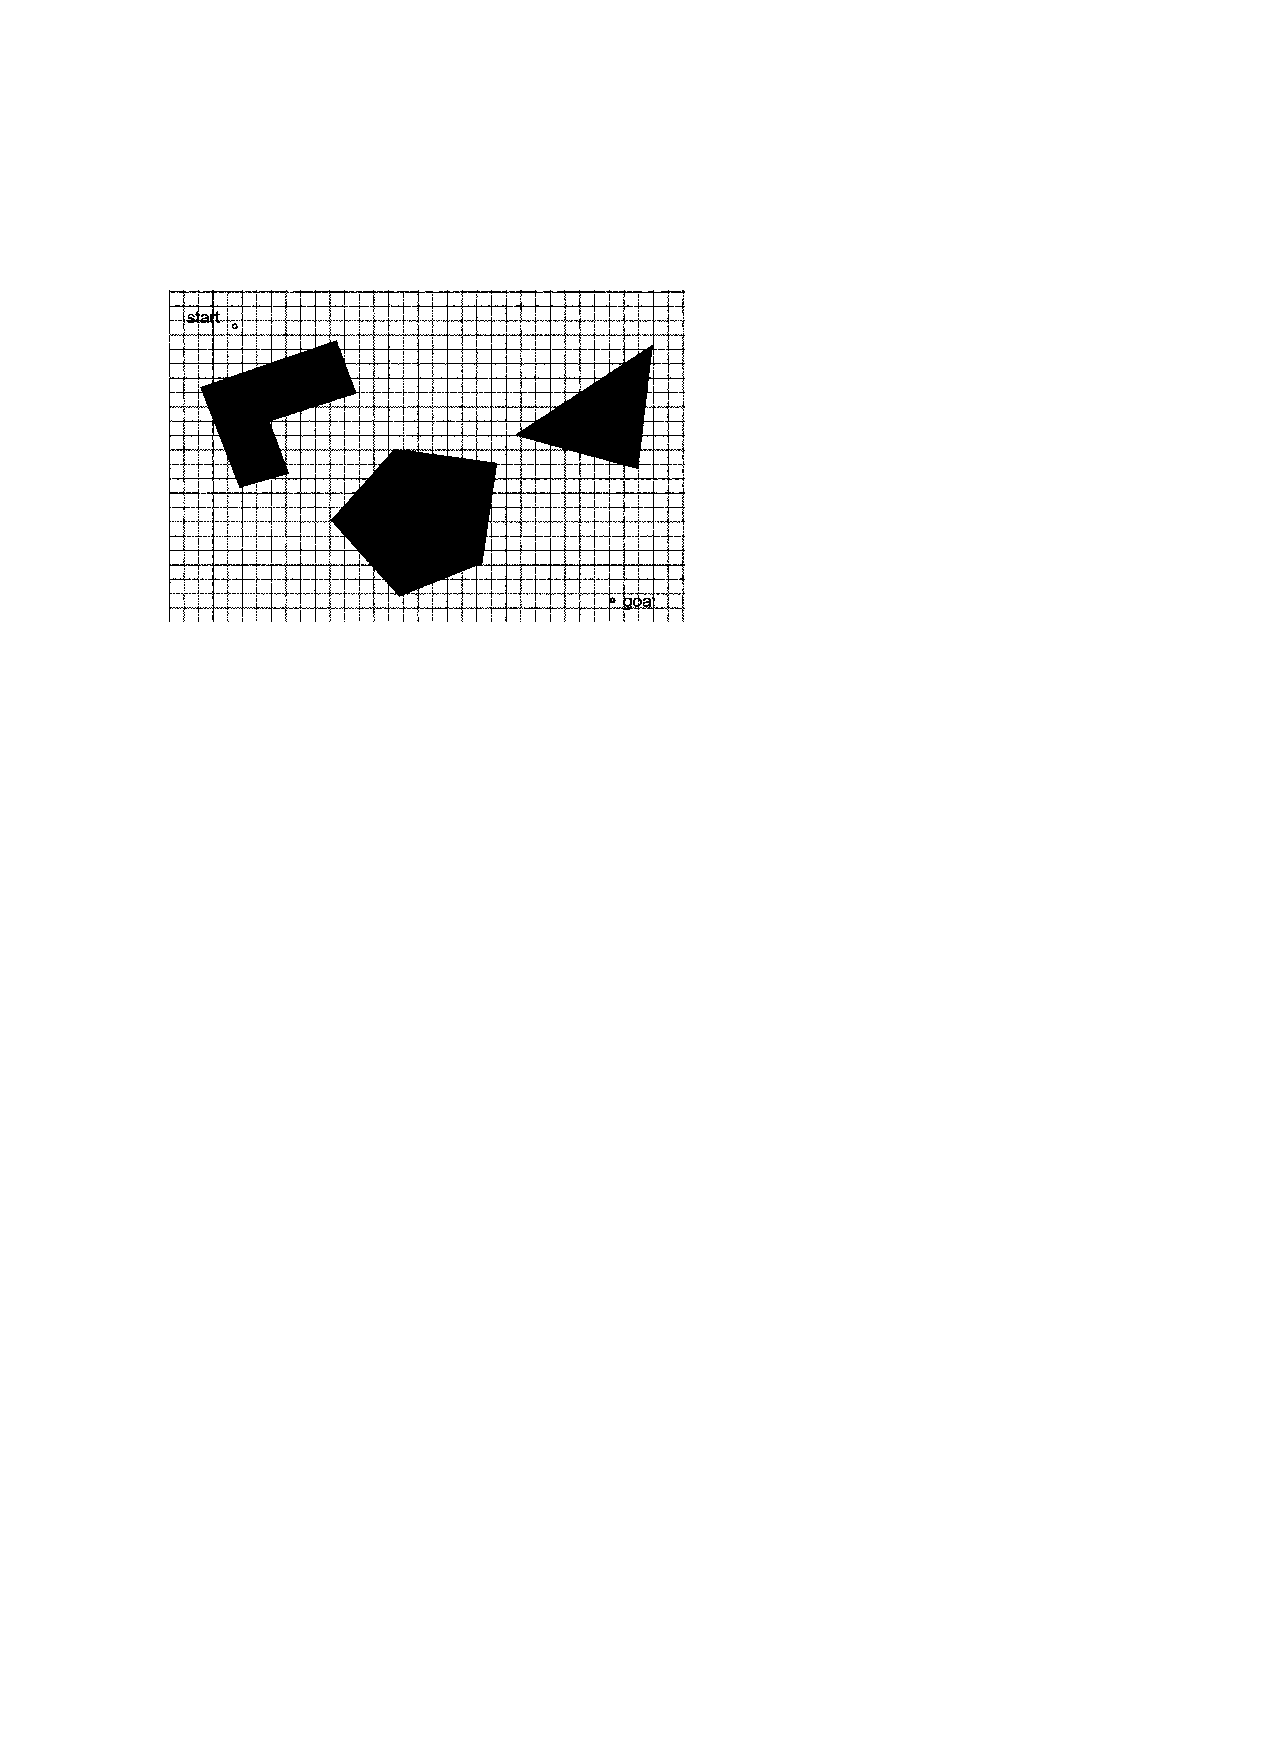
\includegraphics[width=0.4\textwidth]{celdas_fijas1}
  \hspace{0.1cm} 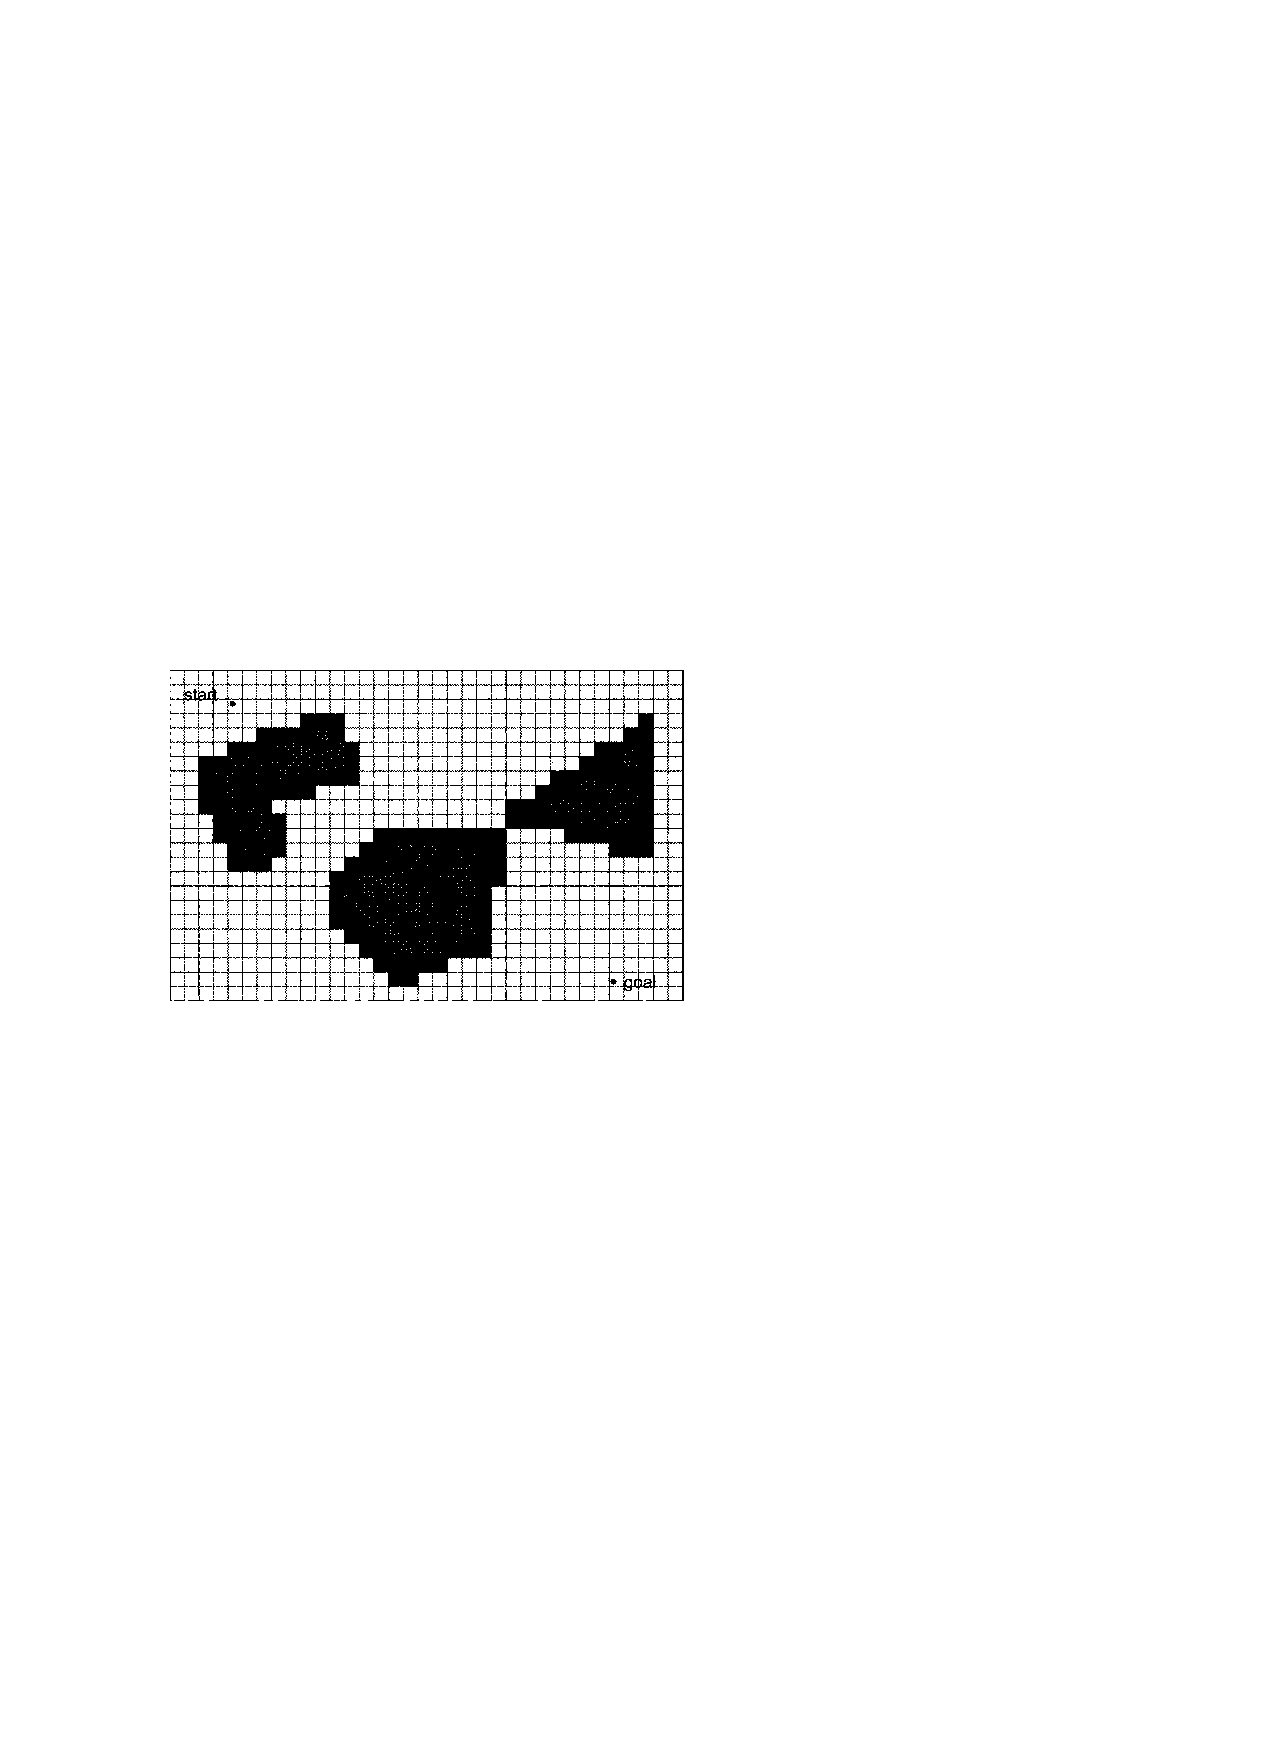
\includegraphics[width=0.4\textwidth]{celdas_fijas2}}  \\
  \caption{Descomposición en celdillas fijas}\label{fg:fijas}
\end{figure}

\begin{figure}[hbt]
  \centering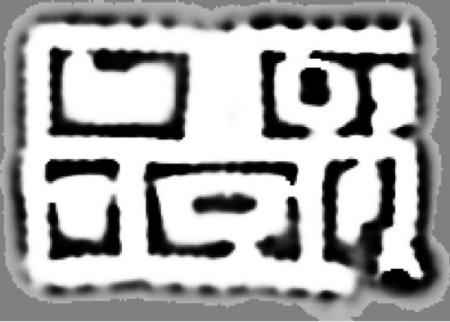
\includegraphics[scale=0.4]{mapa_discretizado}\\
  \caption{Mapa métrico discretizado}\label{fg:discretizado}
\end{figure}


 En este caso no se analiza la pertenencia de cada celdilla a un objeto individual, por lo que aunque el espacio esté discretizado se logra su representación de forma continua. En la figura \ref{fg:discretizado} se puede ver un mapa discretizado o de ocupación de celdillas de un entorno con formas irregulares que haría complicada la representación geométrica.

Este tipo de mapas puede precisar de una alta capacidad de almacenamiento, tanto mayor cuanta más resolución se requiera. Por otra parte, permite representaciones continuas y completas incluso a partir de datos de sensores con mucho ruido como los de ultrasonidos, lo que los hace especialmente prácticos.

\clearpage


El nivel de representación topológico se centra en definir nodos (en ocasiones llamados \emph{lugares distintivos}) y las conexiones entre ellos. Los mapas topológicos a menudo se elaboran a partir de mapas geométricos pero también pueden obtenerse directamente. Un concepto importante en estos modelos es el de nodos adyacentes. Los nodos adyacentes son aquellos que el robot puede alcanzar sucesivamente sin pasar por ningún otro nodo intermedio. Dentro de este nivel son muy comunes las representaciones basadas en el Diagrama de Voronoi o el Gráfico de Voronoi Generalizado (GVG)como las que se presentan en \cite{Choset01} y se muestran en la figura \ref{fg:topologicos}.

\begin{figure}[hbtp]
  % Requires \usepackage{graphicx}
  \centering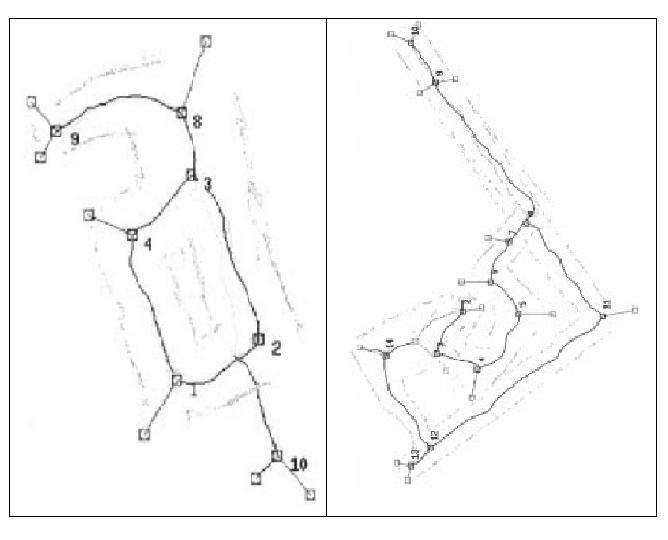
\includegraphics[scale=0.4]{mapas_topologicos}\\
  \caption{Mapas topológicos basados en el diagrama de Voronoi}\label{fg:topologicos}
\end{figure}

%El diagrama de Voronoi es también una forma de hacer frente a la planificación de trayectorias y por ello se trata con más detalle en ese contexto.
Los mapas topológicos tienen un grado de compacidad incluso mayor que los mapas métricos geométricos. Sin embargo, esta representación depende en gran medida de las capacidades sensoriales del robot y da lugar a mapas menos realistas.

La característica fundamental del nivel semántico frente al topológico es que toda la información geométrica se elimina por completo. El resultado es una representación de los lugares más significativos del entorno y sus conexiones, denotados mediante simples etiquetas lingüísticas. En la figura \ref{fg:semantico} se observan los mapas topológico y semántico de un entorno de interiores obtenidos en \cite{Kuipers91}.

\begin{figure}[hbtp]
  % Requires \usepackage{graphicx}
  \centering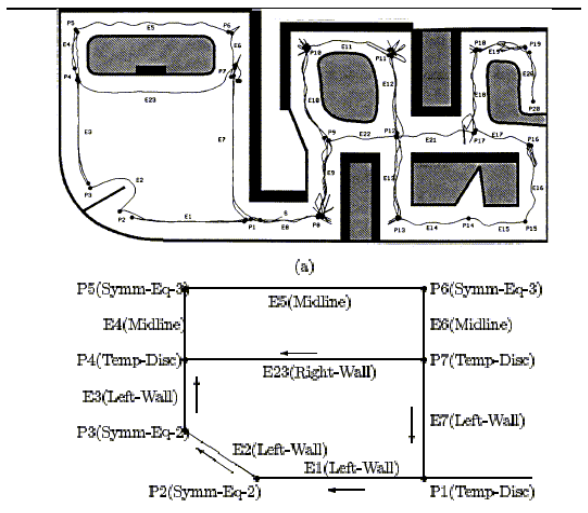
\includegraphics[width=0.5\textwidth]{topo_seman}\\
  \caption{Mapas topológico y semántico}\label{fg:semantico}
\end{figure}

De estos tres niveles, el más utilizado es, sin duda, el métrico. Su principal atractivo es la gran riqueza de su representación, lo que permite una navegación del robot más robusta. Los otros dos niveles de representación suelen construirse a partir del anterior y se utilizan para tareas de planificación de alto nivel. Su compacidad los hará interesantes en entornos estructuralmente complejos o de tamaño superior a los explorados hasta el momento.


 \subsection{SLAM con técnicas probabilísticas}
En cualquier modelo matemático de un sistema existen diversas fuentes de incertidumbre. En los sistemas dinámicos, además, puede haber perturbaciones que afecten al control. Por último, como ya se ha mencionado, los sensores no pueden suministrar información completa y exacta. Estas son algunas de las limitaciones por las que los modelos deterministas resultan insuficientes y por las que se llega al planteamiento de modelos estocásticos.

Desde los años 90 las principales técnicas de construcción de mapas y localización se han fundamentado en la teoría de la probabilidad y, más concretamente, en el teorema de Bayes. Los algoritmos que analizan la solución al problema SLAM desde esta perspectiva son claramente los que mejores resultados han tenido.
La formulación probabilística rigurosa del problema SLAM se conoce comúnmente como Filtro de Bayes y puede considerarse como una generalización temporal del teorema del mismo nombre. El planteamiento se expone a conti\-nuación\cite{Rodriguez-Losada04}.

En la construcción de un mapa por un robot móvil se tienen dos tipos de medidas: las que provienen de los sensores propioceptivos (odometría) y las de los sensores estereoceptivos (observaciones). Se puede suponer sin pérdida de generalidad que estas medidas llegan secuencial y alternativamente en el tiempo:

\begin{equation}\label{eq:medidas-sensores}
    u_{1},z_{1},u_{2},z_{2}...u_{t},z_{t}
\end{equation}

Donde $u$ representa un desplazamiento relativo del robot y $z$ una medida de los sensores externos. El subíndice indica el instante de tiempo al que corresponde cada medida, siendo $t$ el instante actual.
El estado del sistema en el instante $t$ típicamente vendrá dado por la posición del robot $s_{t}$ y la posición de los objetos del mapa $m_{t}$

\begin{equation}\label{eq:estado}
    x_{t}\sim s_{t},m_{t}
\end{equation}

El teorema de Bayes permite conocer la probabilidad de dicho estado condicionada a los datos recogidos hasta ese instante $t$. Hay que destacar que esta función de probabilidad representa cualquier solución probabilista al problema SLAM.

\begin{equation}\label{eq:prob_estado}
    p(x_{t}\mid z^{t},u^{t}) = p(s_{t},m_{t}\mid z^{t},u^{t})=\eta p(z_{t}\mid s_{t},m_{t},z^{t-1},u^{t})p(s_{t},m_{t}\mid z^{t-1}u^{t})
\end{equation}


\begin{eqnarray}
    z^{t} = z_{1},z_{2}...z_{t} \nonumber\\
    u^{t} = u_{1},u_{2}...u_{t}
\end{eqnarray}

Aceptando que el único estado que existe es el definido por $s_{t}$ y $m_{t}$ (hipótesis de Markov), la función de probabilidad puede escribirse nuevamente:

\begin{equation}\label{eq:prob_markov}
    p(x_{t}\mid z^{t},u^{t}) = p(s_{t},m_{t}\mid z^{t},u^{t}) = \eta p(z_{t}\mid s_{t},m_{t})p(s_{t},m_{t}\mid z^{t-1}u^{t})
\end{equation}

El segundo factor puede expresarse en base al teorema de la probabilidad total como:
\begin{eqnarray}\label{eq:prob_total}
  \lefteqn{p(s_{t},m_{t}\mid z^{t-1},u^{t}) =} \\
	&&  \int\int p(s_{t},m_{t}\mid z^{t-1},u^{t},s_{t-1},m_{t-1})
 	\cdot p(s_{t-1},m_{t-1}\mid z^{t-1},u^{t}) ds_{t-1}dm_{t-1}  \nonumber
\end{eqnarray}

Aplicando otra vez la hipótesis de Markov y el hecho de que es lógico pensar que el movimiento del robot es independiente del mapa, se tiene:

\begin{equation}\label{eq:termino2}
    p(s_{t},m_{t}\mid z^{t-1},u^{t}) = \int p(s_{t}\mid u_{t-1},s_{t-1})
    \cdot p(s_{t-1},m\mid z^{t-1},u^{t-1})ds_{t-1}
\end{equation}


Con lo que finalmente queda:
\begin{eqnarray}\label{eq:filtroBayes}
  \lefteqn{p(s_{t},m\mid z^{t},u^{t}) = } \\
  && \eta p(z_{t}\mid s_{t},m_{t})\int p(s_{t}\mid u_{t},s_{t-1})
  \cdot p(s_{t-1},m\mid z^{t-1},u^{t-1})ds_{t-1} \nonumber
\end{eqnarray}

Esta expresión \ref{eq:filtroBayes} es la que se conoce como Filtro de Bayes en el problema SLAM. El problema así planteado puede abordarse recursivamente si se conocen en cada instante las medidas sensoriales de ese instante (con su probabilidad) junto con la función de probabilidad del estado en el instante anterior.
Hacen falta, por lo tanto, dos funciones de probabilidad correspondientes a datos sensoriales: la relativa a la odometría, $p(s_{t}\mid u_{t},s_{t-1})$, y la de las medidas efectuadas por el sistema estereoceptivo, $p(z_{t}\mid s_{t},m_{t})$.

Sin embargo, la ecuación del Filtro de Bayes no puede resolverse ni implementarse directamente sino que es preciso realizar ciertas simplificaciones o suposiciones que dan lugar a los diferentes algoritmos existentes.

El estudio de todos estos algoritmos queda fuera del alcance de este proyecto ya que en él no se hace SLAM propiamente dicho, como se verá en el capítulo correspondiente. La solución adoptada se encuadra dentro de la categoría de métodos de Máxima Probabilidad Incremental. La idea básica del algoritmo así llamado consiste en construir un único mapa según van llegando los datos, sin mantener ninguna noción sobre la incertidumbre del mismo o de la posición del robot en cada instante. Únicamente se determinan la posición y el mapa más probables en cada momento. La principal ventaja del algoritmo es su mayor simplicidad y el menor tiempo de procesamiento y capacidad de almacenamiento que requiere frente a otras soluciones. Sin embargo, no presenta un buen comportamiento a la hora de cerrar bucles dado que al no guardarse ninguna información sobre la incertidumbre del mapa, una estimación realizada no puede corregirse a partir de datos posteriores. Una posible forma de hacer frente a este problema es utilizar algoritmos híbridos. Los algoritmos híbridos ofrecen una aproximación intermedia entre la obtención del mapa más probable sin mantener una noción de la incertidumbre del mismo ni de la posición del robot (algoritmo de Máxima Probabilidad Incremental), y la estimación de la función de probabilidad del mapa completo (solución SLAM-EKF), que conserva la totalidad de la información sobre la incertidumbre. En definitiva lo que hacen este tipo de algoritmos es mantener la incertidumbre en la posición del robot de una u otra forma y estimar el mapa más probable simplificando la ecuación \ref{eq:filtroBayes} para la localización en un mapa dado.


%El sistema de localización implementado no incorpora la construcción simultánea de mapas de los tipos descritos en el capítulo de estado del arte sino que elabora y luego va actualizando un mapa de puntos a partir de las observaciones correspondientes a las medidas del láser. Son los puntos que ya forman parte del mapa los que se utilizan para la localización en cada instante.

\subsection {Localización probabilística basada en mapas}

Entre las técnicas probabilistas de localización destacan especialmente dos tipos de localización: \emph{localización de Markov} y \emph{localización basada en el filtro de Kalman}. El primero de ambos métodos utiliza una distribución de probabilidad explícitamente especificada sobre todas las posibles posiciones del robot en el mapa. No requiere que el robot tenga una posición inicial conocida y permite la relocalización a partir de situaciones ambiguas. Sin embargo, para actualizar la probabilidad de todas las posiciones del espacio de estado hace falta que éste tenga una representación discretizada (mapas de celdillas, mapas topológicos\ldots).

En 1994 se celebró el concurso \emph{1994 American Association for Artificial Intelligence (AAAI) National Robot Contest}, en el que se proporcionaba a los robots participantes un mapa topológico imperfecto del entorno con el cual tenían que conseguir llegar a una determinada habitación establecida como meta. El robot Rinho empleaba en dicho concurso localización de Markov a partir de la construcción de un mapa de celdillas. En la figura \ref{fg:MarkovGrid} pueden verse sus resultados.

\begin{figure}[h]
  % Requires \usepackage{graphicx}
  \centering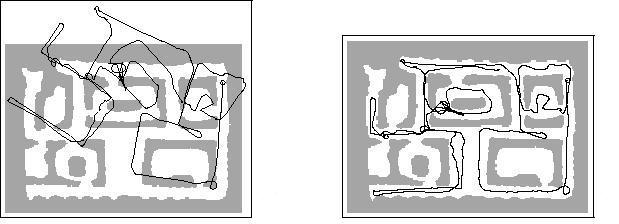
\includegraphics[scale=0.8]{Markov}\\
  \caption{ Trayectorias odométrica y corregida mediante localización de Markov en un mapa de ocupación de celdillas \cite{Fox99}.}\label{fg:MarkovGrid}
\end{figure}

Las técnicas de localización de Markov con mapas topológicos son difíciles de aplicar en entornos no estructurados. En otro tipo de casos, sin embargo, puede ser más adecuado. El ganador de la competición de robots móviles de la AAAI de 1994, llamado Dervish, empleaba localización probabilística de Markov sobre representación topológica del entorno. En la figura \ref{fg:MarkovTop} se muestra un ejemplo de representación topológica de un entorno de oficinas similar al del concurso. Dervish detectaba las puertas cerradas y las puertas abiertas, guardando la información para relacionarla con la conectividad de nodos del mapa. Posteriores desarrollos pueden encontrarse en \cite{Simmons95} y \cite{Kaebling96}.

\begin{figure}[h]
  % Requires \usepackage{graphicx}
  \centering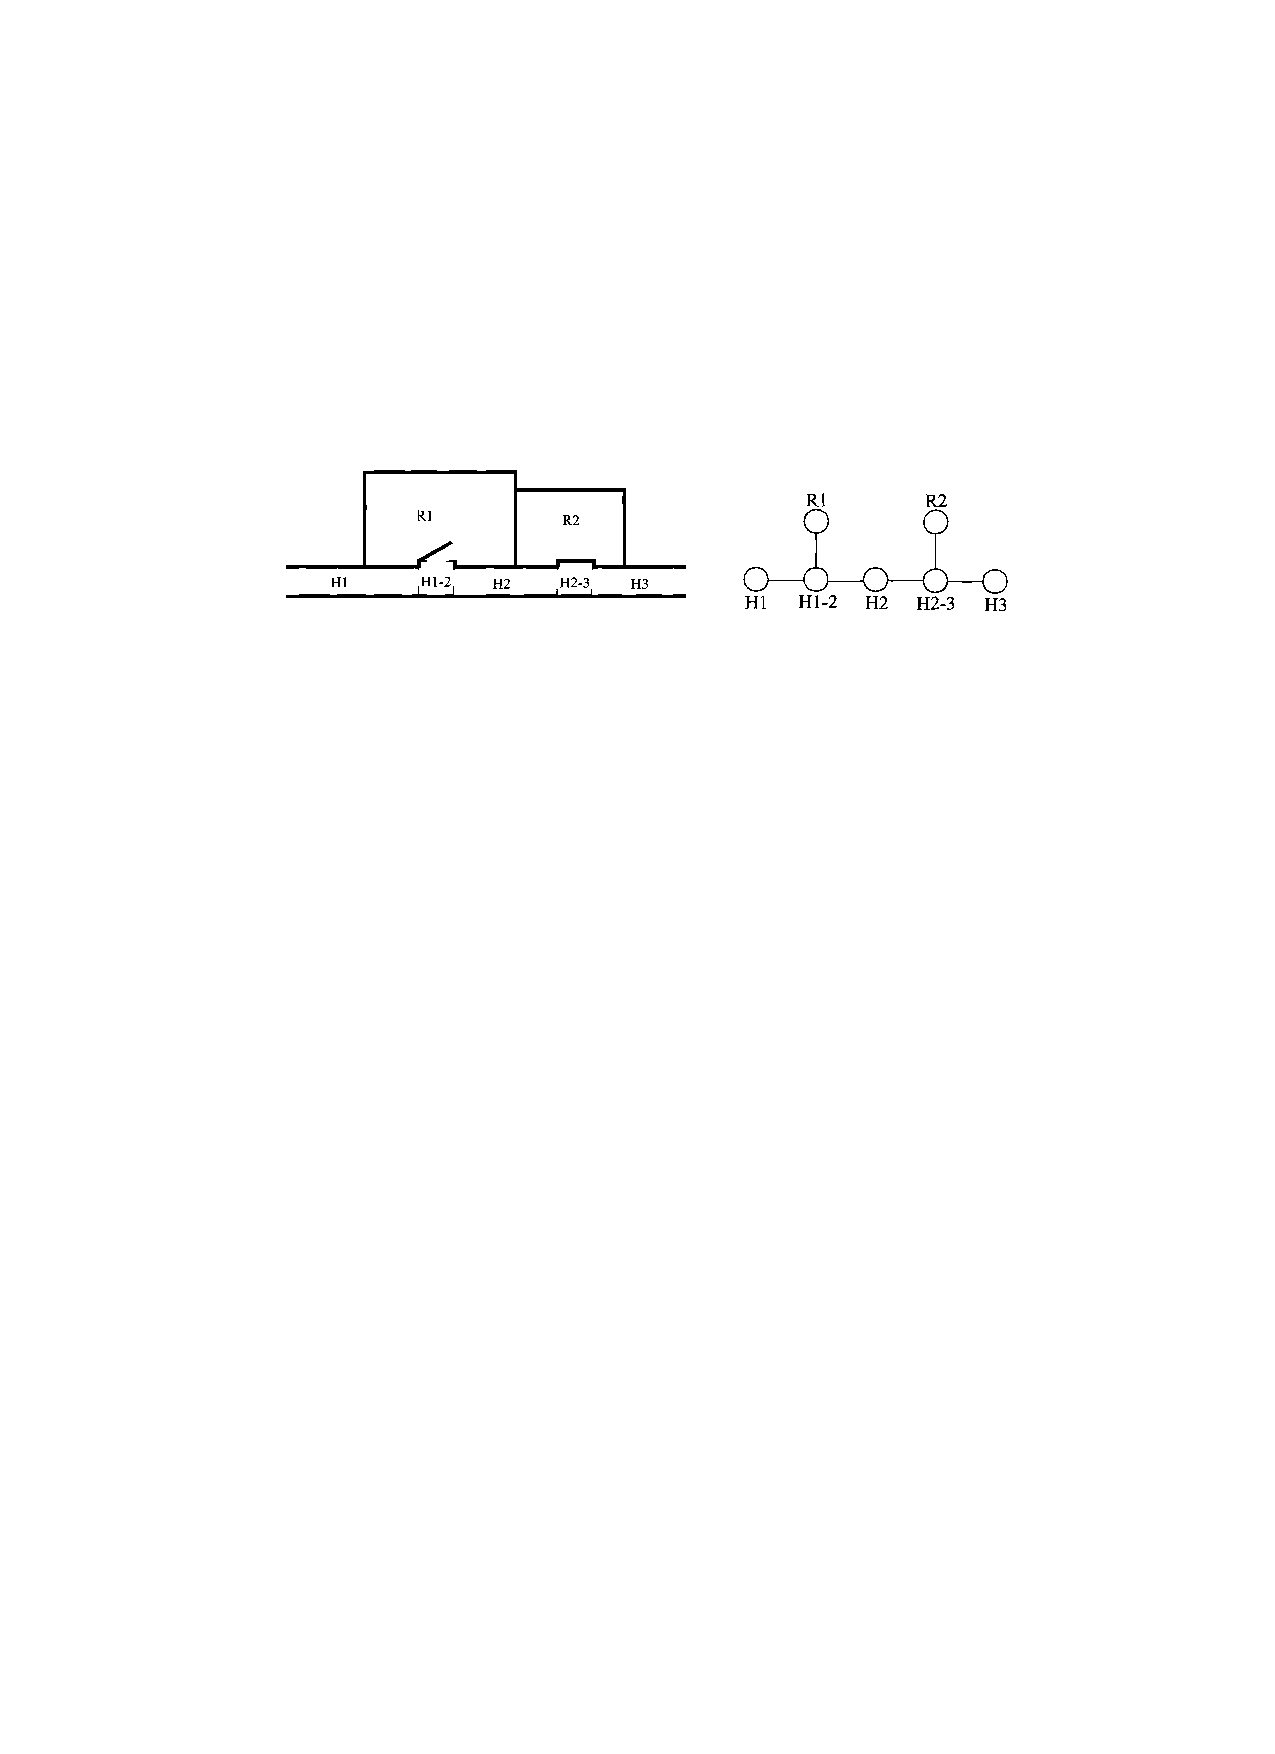
\includegraphics[scale=0.8]{TopoOffice}\\
  \caption{Representación topológica de un entorno de oficina}\label{fg:MarkovTop}
\end{figure}


Otro tipo de localización basada en el método de Markov es la \emph{ localización de Monte Carlo}. En ella, inicialmente se toma al azar  un elevado número de posibles configuraciones hipotéticas para el robot. Con las medidas de los sensores se va actualizando la probabilidad de que cada una de esas configuraciones sea la configuración del robot en ese instante en base a modelos estadísticos mediante aplicación del teorema de Bayes. De un modo similar, cada movimiento incremental del robot se incorpora al cálculo de probabilidades mediante el modelo estadístico de la medida del movimiento. Las configuraciones cuya probabilidad resulta ser muy baja se sustituyen por otras configuraciones aleatorias del espacio de estado.

El filtro de Kalman emplea una representación de densidad de probabilidad Gaussiana de la posición del robot y la asociación de datos para la localización. Es interesante el hecho de que el proceso de localización del filtro de Kalman es el resultante si se aplica al modelo de Markov la suposición de que la incertidumbre en la posición del robot sigue una distribución normal.

Las principales ventajas de la localización mediante filtro de Kalman son su precisión y eficiencia cuando se conoce la posición de partida en el movimiento del robot, el poder aplicarse con modelos de representación del entorno continuos (mapas geométricos) y las menores necesidades de tiempo y memoria respecto a la localización de Markov. El mayor inconveniente que presenta es la posibilidad de que el robot quede completamente perdido si el error en su movimiento es demasiado grande (como resultado del choque con un obstáculo, por ejemplo).

\subsection {Filtro de Kalman}
La localización basada en el filtro de Kalman es la más extendido en la literatura y en implementaciones prácticas y debido a sus buenas propiedades, apropiadas para la mayor parte de aplicaciones, es la que se ha utilizado en el desarrollo de este proyecto.

\subsubsection {Conceptos introductorios}
El filtro de Kalman es un algoritmo recursivo óptimo para procesar información\cite{Maybeck79}. Combina la totalidad de la información disponible, ponderándola según su grado de incertidumbre, para realizar la estimación de las variables que definan el estado del sistema. El funcionamiento del filtro requiere el conocimiento de la dinámica del sistema, así como de los modelos estadísticos del ruido en las medidas de los sensores y de la incertidumbre inicial del modelo del sistema. Al tratarse de un algoritmo recursivo, cada estimación se efectúa a partir de la anterior y de la nueva información disponible, sin que sea preciso almacenar todos los datos previos.

El filtro de Kalman permite minimizar el error en la estimación de las variables de interés cuando el modelo es lineal y la incertidumbre del sistema y de las medidas de los sensores es ruido blanco gaussiano. En esta situación, la función de densidad de probabilidad de cada variable a analizar condicionada a las medidas tomadas es tal que la media, la moda y la mediana coinciden, lo que evita cualquier posible conflicto a la hora de determinar cuál es la mejor estimación.
Las hipótesis aceptadas pueden parecer altamente restrictivas pero hacen posible la resolución matemática del problema y se acercan bastante bien a la realidad en la mayoría de los casos. En otros, sin embargo, han de contemplarse algunas variaciones y resulta de utilidad el llamado filtro extendido de Kalman (EKF).

\subsubsection{Ecuaciones para sistemas dinámicos}
A continuación se muestran las ecuaciones que definen el comportamiento del filtro de Kalman aplicado a sistemas dinámicos\cite{Schutter99}.

La relación entre cada una de las medidas tomadas en un instante y el estado del sistema es del tipo:
\begin{equation}\label{eq:measurement}
   z_{k} = H_{k}x_{k}+\rho_{m}
\end{equation}
Con z vector de medidas, x vector de estado y $\rho_{m}$ ruido gaussiano en las medidas, con media nula y matriz de covarianza $R_{k}$ ó $R$ si ésta es constante en el tiempo.

Se considera que la evolución del sistema sigue el siguiente modelo de estado lineal:
\begin{equation}\label{eq:model}
    x_{k} = Ax_{k-1}+Bu_{k-1}+\rho_{\rho},
\end{equation}
donde A es la matriz de estado; B, la matriz de entrada; $u_{k-1}$, el vector de entrada en el instante k-1 y $\rho_{\rho}$ representa la incertidumbre del proceso (con matriz de covarianza $Q_{p}$, o $Q_{p_{k-1}}$ si es variable con el tiempo).


\textbf{Etapa de predicción}
Así, la \emph{predicción del estado}, $\tilde{x}_{k}$, vendrá dada por:
\begin{equation}\label{eq:x_prediction}
    \tilde{x}_{k} = A\hat{x}_{k-1}+Bu_{k-1},
\end{equation}

siendo $\hat{x}_{k-1}$ la estimación del estado en el instante k-1.

Si la entrada $u$ se conoce con exactitud, el error de predicción dado por la diferencia entre \ref{eq:x_prediction} y \ref{eq:model} será:
\begin{equation}\label{eq:prediction_error}
    \tilde{x}_{k}-x_{k} = A(\hat{x}_{k-1}-x_{k-1})- \rho_{\rho}
\end{equation}

y la matriz de covarianza de $x_{k}$ queda:
\begin{equation}\label{eq:P_prediction}
    \tilde{P}_{k} = A\hat{P}_{k-1}A^{T}+Q_{p_{k-1}}
\end{equation}


\textbf{Etapa de corrección}
La solución de mínimos cuadrados entre las medidas y las medidas esperadas es:
\begin{equation}\label{eq:x_estimation}
    \hat{x}_{k} = \tilde{x}_{k}+K_{k}(z_{k}-H_{k}\tilde{x}_{k})
\end{equation}

\begin{equation}\label{eq:P_estimation}
    \hat{P}_{k} = (I-K_{k}H_{k})\tilde{P}_{k}
\end{equation}

con
\begin{equation}\label{eq:K}
    K_{k} = \tilde{P}_{k}H_{k}^{T}S_{k}^{-1}
\end{equation}

\begin{equation}\label{eq:S}
    S_{k} = R_{k}+H_{k}\tilde{P}_{k}H_{k}^{T}
\end{equation}

Estas ecuaciones constituyen el llamado filtro \emph{dinámico} de Kalman.
La matriz $K_{k}$ se denomina \emph{ganancia de Kalman}.
La diferencia entre las medidas en k y sus valores esperados, $v_{k} = z_{k}-H_{k}\tilde{x}_{k}$, se conoce como la \emph{innovación} del proceso y la matriz $S$ corresponde a su matriz de covarianza.

El filtro de Kalman \emph{estático} es un caso particular del anterior y se obtiene a partir de estas ecuaciones haciendo $A = I$, $B = 0$ y $Q_{p} = 0$.

\subsection{Filtro Extendido de Kalman}
La principal aportación de este algoritmo respecto al del filtro de Kalman convencional es su extensión a sistemas no lineales. También permite incorporar los casos en los que la relación entre el estado y las medidas de los sensores externos no puede definirse de forma explícita. La convergencia del EKF depende de diversos factores como pueden ser la estimación inicial, las no linealidades de las ecuaciones, el orden en que se procesan las medidas...De este modo, no existe prueba formal de la convergencia del algoritmo, sino tan solo ciertos tests de consistencia que evalúan el comportamiento del mismo en cada caso.

\subsubsection{Ecuaciones para sistemas no lineales}
Las ecuaciones del medida \ref{eq:measurement} y de estado \ref{eq:model}, frecuentemente presentan carácter no lineal:
\begin{equation}\label{eq:medida_nolineal}
    z = h(x)+\rho_{m}
\end{equation}

\begin{equation}\label{eq:estado_nolineal}
    x_{k} = f(x_{k-1},u_{k-1})+\rho_{\rho},
\end{equation}

cuyas ecuaciones linealizadas en la estimación más reciente son:
\begin{equation}\label{eq:medida_linealizada}
    z = h(\tilde{x}_{k})+\frac{\delta h}{\delta x}|_{ _{\tilde{x}_k}} (x-\tilde{x}_{k})+\rho_{m}
\end{equation}

\begin{equation}\label{eq:estado_linealizada}
    x_{k} = f(\hat{x}_{k-1},u_{k-1})+\frac{\delta f}{\delta x}\mid _{_{\hat{x}_k-1}} (x_{k-1}-\hat{x}_{k-1})+\rho_{\rho}
\end{equation}

Con ello, las ecuaciones del EKF se obtienen de la siguiente manera:


\textbf{Etapa de predicción}
\begin{equation}\label{eq:x_predictionEKF}
    \tilde{x}_{k} = f(\hat{x}_{k-1},u_{k-1})
\end{equation}

Sustituyendo $A$ por $\frac{\delta f}{\delta x}\mid _{\hat{x}_k-1}$ en \ref{eq:P_prediction}:
\begin{equation}\label{eq:P_predictionEKF}
    \tilde{P}_{k} = (\frac{\delta f}{\delta x}\mid_{ _{\hat{x}_k-1}}) \hat{P}_{k-1} (\frac{\delta f}{\delta x}\mid_{ _{\hat{x}_k-1}})^{^{T}}+Q_{p_{k-1}}
\end{equation}


\textbf{Etapa de corrección}
Empleando la ecuación de medida no lineal para realizar la predicción de las medidas, \ref{eq:x_estimation} pasa a ser:
\begin{equation}\label{eq:x_estimationEKF}
    \hat{x}_{k} = \tilde{x}_{k}+K_{k}(z_{k}-h(\tilde{x}_{k})),
\end{equation}
donde se aprecia que la innovación es, en este caso, $v_{k} = z_{k}-h(\tilde{x}_{k})$.

Para completar el algoritmo,  \ref{eq:P_estimation}, \ref{eq:K}, \ref{eq:S} se modifican mediante $H_{k}\leftarrow \frac{\delta h}{\delta x}\mid_{\hat{x}_{k-1}}$:

\begin{equation}\label{eq:P_estimationEKF}
    \hat{P}_{k} = (I-K_{k}\frac{\delta h}{\delta x}\mid _{_{\hat{x}_{k-1}}})\tilde{P}_{k}
\end{equation}

\begin{equation}\label{eq:KEKF}
    K_{k} = \tilde{P}_{k}(\frac{\delta h}{\delta x}\mid _{_{\hat{x}_{k-1}}})^{T}S_{k}^{-1}
\end{equation}

\begin{equation}\label{eq:SEKF}
    S_{k} = R_{k}+(\frac{\delta h}{\delta x}\mid _{\hat{x}_{k-1}})\tilde{P}_{k} (\frac{\delta h}{\delta x}\mid _{_{\hat{x}_{k-1}}})^{T}
\end{equation}

\subsubsection{Ecuaciones para el caso de ecuación de medida en forma implícita}

No siempre es posible despejar $z$ en la forma de \ref{eq:measurement}. En su lugar, a veces sólo se dispone de ecuaciones implícitas del tipo:
\begin{equation}\label{eq:implicit}
    h(x,z)+\rho_{m}=c,
\end{equation}
con $c$ vector de constantes.
En este caso, las ecuaciones anteriores varían del siguiente modo:


\textbf{Etapa de predicción}
No se ve afectada, ya que en ella no influyen las medidas estereoceptivas.


\textbf{Etapa de corrección}
Al ser ahora la innovación $v_{k}=c-h(\tilde{x}_{k},z_{k})$, la ecuación \ref{eq:x_estimationEKF} se transforma en:
\begin{equation}\label{eq:x_estimationIm}
    \hat{x}_{k} = \tilde{x}_{k}+K_{k}(c-h(\tilde{x}_{k},z_{k}))
\end{equation}

En las expresiones \ref{eq:P_estimation}, \ref{eq:K}, \ref{eq:S} ha de efectuarse el cambio $H_{k}\leftarrow \frac{\delta h}{\delta x}\mid_{\tilde{x}_{k},z_{k}}$. La matriz $R_{k}$ ha de sustituirse por $(\frac{\delta h}{\delta z} \mid _{\tilde{x}_{k},z_{k}}) R_{k} (\frac{\delta h}{\delta z} \mid _{\tilde{x}_{k},z_{k}})^{T}$.

 \begin{equation}\label{eq:P_estimationEKF_im}
    \hat{P}_{k} = (I-K_{k}\frac{\delta h}{\delta x}\mid_{\tilde{x}_{k},z_{k}})\tilde{P}_{k}
\end{equation}

\begin{equation}\label{eq:KEKF_im}
    K_{k} = \tilde{P}_{k}(\frac{\delta h}{\delta x}\mid_{\tilde{x}_{k},z_{k}})^{T}S_{k}^{-1}
\end{equation}

\begin{equation}\label{eq:SEKF_im}
    S_{k} = (\frac{\delta h}{\delta z} \mid _{\tilde{x}_{k},z_{k}}) R_{k} (\frac{\delta h}{\delta z} \mid _{\tilde{x}_{k},z_{k}})^{T}+(\frac{\delta h}{\delta x}\mid_{\tilde{x}_{k},z_{k}})\tilde{P}_{k} (\frac{\delta h}{\delta x}\mid_{\tilde{x}_{k},z_{k}})^{T}
\end{equation}

Ya se ha comentado la complejidad que puede entrañar la asociación de datos. Además, el hecho de que ésta se haga correctamente es de una gran importancia para el buen funcionamiento del algoritmo.De hecho, es sabido que una asociación de datos errónea conduce fácilmente a la rápida divergencia del mapa tras ser aplicada en la etapa de corrección, sin posibilidad de que el error pueda ser subsanado posteriormente.

La estrategia más ampliamente utilizada consiste en calcular la llamada distancia de Mahalanobis de la observación a todos los objetos del mapa y tomar aquella que sea menor. Es lo que se conoce como la técnica del \emph{Neirest Neighbour }(ND), pues se empareja cada observación con el punto del mapa estadísticamente más cercano. Para comprobar que una innovación es consistente con el modelo lo que se hace es calcular la distancia de Mahalanobis de la misma y determinar si este valor de la adecuación de la medida al estado se encuentra dentro de un intervalo de confianza escogido. El cuadrado de la distancia de Mahalanobis se calcula mediante $v_{k}^{T}S_{k}^{-1}v_{k}$ y también recibe el nombre de \emph{Normalised Innovation Squared}, $NIS_{k}$. Este parámetro tiene distribución $\chi^{2}$ con tantos grados de libertad como medidas independientes haya en el vector de medidas $z_{k}$, con lo que la decisión de aceptar o rechazar la medida se hará en base a:
\begin{equation}\label{eq:mahalanobis}
    v_{k}^{T}S_{k}^{-1}v_{k}<\chi^{2}_{dim(v_{k}),\alpha = confianza}
\end{equation}

Otras forma más robusta de realizar la asociación de datos es el test de Compatibilidad Conjunta o "Joint Compatibility" (JC), pero resulta más difícil de implementar y tiene un coste computacional mayor. Esta estrategia ya no considera cada una de las asociaciones independientemente, siendo aplicable en el caso de que puedan realizarse varias observaciones a la vez o bien si cada una de ellas pueda asociarse a varios puntos del mapa previo. En general se suele aplicar la ecuación \ref{eq:mahalanobis} para establecer los emparejamientos iniciales y posteriormente se calcula una distancia de Mahalanobis conjunta mediante el vector acumulado de innovaciones y la matriz conjunta de varianzas y covarianzas de las mismas, de modo que pueda determinarse si las asociaciones anteriores pueden realizarse de forma simultánea. Para cada emparejamiento individual, cabe la posibilidad de que sea compatible con el resto o no, por lo que el coste computacional se incrementa exponencialmente y será O=($2^{q}$), con $q$ igual al número de dichos emparejamientos individuales (aquellos que satisfacen \ref{eq:mahalanobis}).

En el proyecto se ha utilizado la primera alternativa, ya que, aunque se realizan observaciones simultáneamente, al emplearse mapas de puntos no es muy probable la asociación múltiple a varios objetos del mismo mientras el error en la posición sea inferior a la distancia entre puntos del mapa. Como no se tienen muchos errores, esta opción es mejor para no incurrir en un aumento extra del tiempo de procesamiento. Deberá tenerse en cuenta, en todo caso, que la asociación de datos resulta menos fiable a medida que aumenta la incertidumbre en la posición de las características observadas, como ocurre cuando el robot revisita zonas mapeadas con anterioridad, tras cerrar algún bucle.

